\subsection{Dạng 1. Tính số đo góc}
\noindent

\begin{bt}
	Trên đường thẳng $xy$ lấy điểm $O$.
	Trên cùng một nửa mặt phẳng có bờ là đường thẳng $xy$, vẽ hai tia $Om$ và $On$ sao cho
	hai góc $\widehat{xOm}$ và $\widehat{yOn}$ là hai góc phụ nhau và
	$\widehat{xOm}=56^\circ$.
	
	\begin{enumerate}[label=\alph*)]
		\item Tính góc $\widehat{yOn}$.
		
		\item Tính góc kề bù với góc $\widehat{xOm}$.
		
		\item Tính góc kề bù với góc $\widehat{yOn}$.
		
		\item Vẽ tia $Ot$ là tia phân giác của góc $\widehat{mOn}$.
		Tính số đo góc $\widehat{tOy}$.
	\end{enumerate}
\end{bt}

\begin{bt}
	Cho $\widehat{AOB}$ và $\widehat{BOC}$ là hai góc kề bù. Biết
	$\widehat{BOC}=5\widehat{AOB}$.
	
	\begin{enumerate}[label=\alph*)]
		\item Tính số đo mỗi góc.
		\item Gọi $OD$ là tia phân giác của $\widehat{BOC}$. Tính số đo $\widehat{AOD}$.
	\end{enumerate}
\end{bt}


\subsection{Dạng 2. Chứng minh một tia là tia phân giác}
\noindent
\begin{bt}
	Trên cùng một nửa mặt phẳng có bờ chứa tia $Ox$, vẽ hai tia $Oy$ và $Ot$
	sao cho $\widehat{xOy}=30^\circ$ và $\widehat{xOt}=60^\circ$.
	
	\begin{enumerate}[label=\alph*)]
		\item Chứng minh tia $Oy$ nằm giữa hai tia $Ox$ và $Ot$.
		
		\item Tính số đo $\widehat{yOt}$. Từ đó chứng minh $Oy$ là tia phân giác
		của $\widehat{xOt}$.
		
		\item Gọi $Om$ là tia đối của tia $Ox$ và $Oz$ là tia phân giác của
		$\widehat{mOt}$. Tính số đo $\widehat{tOz}$.
		
		\item Chứng minh $Ot$ là tia phân giác của $\widehat{xOz}$.
	\end{enumerate}
\end{bt}
\begin{bt}
	Cho $\widehat{xOy}=120^\circ$. Bên trong $\widehat{xOy}$, vẽ tia $Om$
	sao cho $\widehat{yOm}=30^\circ$ và vẽ tia $On$ sao cho
	$\widehat{yOn}=90^\circ$.
	
	\begin{enumerate}[label=\alph*)]
		\item So sánh số đo $\widehat{xOn}$ và $\widehat{yOm}$.
		
		\item Gọi $Ot$ là tia phân giác của $\widehat{xOy}$. Chứng minh rằng
		$Ot$ cũng là tia phân giác của $\widehat{mOn}$.
	\end{enumerate}
\end{bt}
\newpage
\noindent
\subsection{Dạng 3. Hai tia đối nhau -- hai góc đối đỉnh}
\begin{ghinho}
	\textbf{Nếu đề không chỉ rõ đó là hai góc đối đỉnh thì
	\textcolor{red!75!black}{phải giải thích} trước khi sử dụng.}
\end{ghinho}

\begin{bt}
	Cho góc bẹt $\widehat{xOy}$. Trên cùng một nửa mặt phẳng có bờ là đường
	thẳng $xy$, vẽ hai tia $Ot$, $Oz$; trên nửa mặt phẳng đối diện, vẽ tia
	$Oh$ sao cho $\widehat{xOz}=\widehat{yOt}=\widehat{xOh}=50^\circ.$
	Hai góc $\widehat{xOh}$ và $\widehat{yOt}$ có phải là hai góc đối đỉnh
	không? Vì sao?

\begingroup
	\bfseries\itshape\boldmath
	Gợi ý: Dùng tính chất bắc cầu để chứng minh
	\[
		\begin{aligned}
			a+b &= 180^\circ\\
			c+b &= 180^\circ
		\end{aligned}
		\quad\Longrightarrow\quad a=c.
	\]
\endgroup
\end{bt}

\begin{bt}
	Cho hai đường thẳng $xy$ và $x'y'$ cắt nhau tại $O$. Vẽ tia $Oz$ là
	tia phân giác của $\widehat{x'Oy}$ và tia $Ot$ là tia phân giác của
	$\widehat{xOy'}$.
	
	\begin{enumerate}[label=\alph*)]
		\item Chứng minh $\widehat{xOt}=\widehat{x'Oz}$.
		
		\item Chứng minh $\widehat{xOt}$ và $\widehat{yOz}$ là hai góc đối đỉnh.
	\end{enumerate}
\end{bt}

\begin{bt}
	Cho hai đường thẳng $a$ và $b$ cắt nhau tại $O$, tạo thành bốn góc
	$\widehat{O_1}$, $\widehat{O_2}$, $\widehat{O_3}$, $\widehat{O_4}$
	như hình dưới đây. Tính số đo các góc trong mỗi trường hợp sau:

	\begin{flushright}
		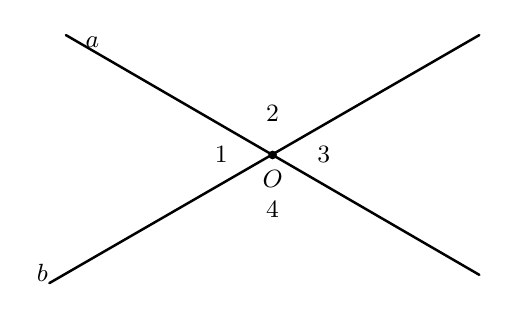
\begin{tikzpicture}[
			scale=1.05,
			line cap=round,
			line join=round,
			font=\small
		]
			\coordinate (O) at (0,0);

			% Hai đường thẳng a và b
			\draw[line width=0.9pt] (-2.5,1.45)--(2.5,-1.45);
			\draw[line width=0.9pt] (-2.7,-1.55)--(2.5,1.45);

			% Giao điểm và tên đỉnh
			\fill (O) circle (1.5pt);
			\node[below=2pt] at (O) {$O$};

			% Số thứ tự của bốn góc
			\node at (-0.62,0) {$1$};
			\node at (0,0.50) {$2$};
			\node at (0.62,0) {$3$};
			\node at (0,-0.66) {$4$};

			% Tên hai đường thẳng
			\node[above right] at (-2.38,1.18) {$a$};
			\node[left] at (-2.6,-1.42) {$b$};
		\end{tikzpicture}
	\end{flushright}

	\begin{enumerate}[label=\alph*)]
		\item $\widehat{O_1}=\dfrac{1}{2}\widehat{O_2}$.
		
		\item $\widehat{O_1}-\widehat{O_2}=40^\circ$.
		
		\item $\widehat{O_1}+\widehat{O_3}
		=\dfrac{1}{2}\left(\widehat{O_2}+\widehat{O_4}\right)$.
	\end{enumerate}
\end{bt}

\subsection{Dạng 4. Hai đường thẳng vuông góc}

\begin{bt}
	Cho hai góc kề $\widehat{AOB}$ và $\widehat{BOC}$ có tổng bằng
	$160^\circ$, biết $\widehat{AOB}=7\widehat{BOC}$.
	
	\begin{enumerate}[label=\alph*)]
		\item Tính số đo mỗi góc.
		
		\item Trong $\widehat{AOC}$, vẽ tia $OD\perp OC$. Chứng minh rằng
		$OD$ là tia phân giác của $\widehat{AOB}$.
		
		\item Vẽ tia $OC'$ là tia đối của tia $OC$. Chứng minh rằng
		$\widehat{AOC}=\widehat{BOC'}$.
	\end{enumerate}

	\begin{center}
		\begin{tikzpicture}[
			scale=1.05,
			line cap=round,
			line join=round,
			font=\small,
			every node/.style={inner sep=1.5pt}
		]
			\coordinate (O)  at (0,0);
			\coordinate (A)  at (180:3.0);
			\coordinate (B)  at (40:2.8);
			\coordinate (C)  at (20:3.0);
			\coordinate (D)  at (110:2.8);
			\coordinate (Cp) at (200:2.2);

			\draw[mauChuDao,line width=0.9pt] (O)--(A);
			\draw[mauChuDao,line width=0.9pt] (O)--(B);
			\draw[mauChuDao,line width=0.9pt] (Cp)--(O)--(C);
			\draw[mauChuDao,line width=0.9pt] (O)--(D);
			\pic[draw=mauChuDao,angle radius=7pt] {right angle=D--O--C};

			\fill (O) circle (1.4pt);
			\node[below] at (O) {$O$};
			\node[left] at (A) {$A$};
			\node[above right] at (B) {$B$};
			\node[above right] at (C) {$C$};
			\node[above left] at (D) {$D$};
			\node[below left] at (Cp) {$C'$};

			\foreach \P in {A,B,C,D,Cp}{
				\fill[red!75!black] (\P) circle (1.3pt);
			}
		\end{tikzpicture}
	\end{center}
\end{bt}

\begin{bt}
	Cho góc tù $\widehat{MOB}$. Vẽ tia $OC$ nằm trong góc đó. Biết
	$\widehat{MOC}+\widehat{MOB}=180^\circ$. Vẽ tia $ON$ là tia phân giác
	của $\widehat{BOC}$. Chứng minh rằng:
	
	\begin{enumerate}[label=\alph*)]
		\item $\widehat{BOC}=180^\circ-2\widehat{MOC}$.
		
		\item $OM\perp ON$.
	\end{enumerate}
\end{bt}

\subsection{Dạng 5. Bài tập tổng hợp}

\begin{bt}
	Vẽ hai góc kề bù $\widehat{xOy}$ và $\widehat{yOx'}$, biết
	$\widehat{xOy}=70^\circ$. Gọi $Ot$ và $Ot'$ lần lượt là các tia phân giác
	của $\widehat{xOy}$ và $\widehat{x'Oy}$.
	
	\begin{enumerate}[label=\alph*)]
		\item Tính $\widehat{yOx'}$ và $\widehat{xOt'}$.
		
		\item Tính $\widehat{tOt'}$. Từ đó cho biết hai tia $Ot$ và $Ot'$ có
		vuông góc với nhau không.
	\end{enumerate}
\end{bt}

\begin{bt}
	Cho hai đường thẳng $xx'$ và $yy'$ cắt nhau tại $O$, biết
	$\widehat{xOy}=40^\circ$. Các tia $Om$ và $On$ lần lượt là tia phân giác
	của $\widehat{xOy}$ và $\widehat{x'Oy'}$.
	
	\begin{enumerate}[label=\alph*)]
		\item Tính số đo các góc $\widehat{xOy'}$, $\widehat{x'Oy}$ và
		$\widehat{x'Oy'}$.
		
		\item Chứng minh $Om$ và $On$ là hai tia đối nhau.
	\end{enumerate}
\end{bt}

\begin{bt}
	Cho $\widehat{AOB}=150^\circ$. Về phía ngoài của $\widehat{AOB}$, vẽ
	hai tia $OC$ và $OD$ sao cho $OA\perp OC$ và $OB\perp OD$. Gọi $Ox$ là
	tia phân giác của $\widehat{AOB}$, $Oy$ là tia đối của tia $Ox$.
	
	\begin{enumerate}[label=\alph*)]
		\item Chứng minh $Oy$ là tia phân giác của $\widehat{COD}$.
		
		\item So sánh $\widehat{xOC}$ và $\widehat{yOB}$.
	\end{enumerate}

	\begin{flushright}
		\begin{tikzpicture}[
			scale=0.9,
			line cap=round,
			line join=round,
			font=\small,
			every node/.style={inner sep=1.5pt}
		]
			\coordinate (O) at (0,0);
			\coordinate (A) at (180:3.2);
			\coordinate (B) at (30:3.0);
			\coordinate (C) at (270:2.7);
			\coordinate (D) at (300:2.9);
			\coordinate (X) at (105:2.7);
			\coordinate (Y) at (285:2.4);

			\draw[mauChuDao,line width=0.9pt] (O)--(A);
			\draw[mauChuDao,line width=0.9pt] (O)--(B);
			\draw[mauChuDao,line width=0.9pt] (O)--(C);
			\draw[mauChuDao,line width=0.9pt] (O)--(D);
			\draw[mauChuDao,line width=0.9pt] (O)--(X);
			\draw[mauChuDao,line width=0.9pt] (O)--(Y);

			\pic[draw=mauChuDao,angle radius=7pt] {right angle=A--O--C};
			\pic[draw=mauChuDao,angle radius=7pt] {right angle=B--O--D};

			\fill (O) circle (1.4pt);
			\node[above left] at (O) {$O$};
			\node[left] at (A) {$A$};
			\node[above right] at (B) {$B$};
			\node[below] at (C) {$C$};
			\node[right] at (D) {$D$};
			\node[above] at (X) {$x$};
			\node[below] at (Y) {$y$};

			\foreach \P in {A,B,C,D,X,Y}{
				\fill[red!75!black] (\P) circle (1.3pt);
			}
		\end{tikzpicture}
	\end{flushright}
\end{bt}
